% !TEX root = your-paper.tex

\pdfoutput=1
\documentclass{article}


% alptex + small aesthetic tweaks + some extra math defs
\input{preamble/preamble.tex}
\input{preamble/preamble_math}
\input{preamble/definitions_basic}

% bibtex import + some code to strip away useless bib info (volume number, isbn, and the ilk), and to standardize capitalization
% warning: the arxiv uses an outdated bibtex, which causes cryptic and frustrating upload errors 
% easiest solution: install whatever current arxiv texlive is from ftp://tug.org/historic/systems/texlive/ (download the ISO) and compile using this versions pdflatex and bibtex
% alternatively, look upon https://github.com/plk/biblatex/wiki/biblatex-and-the-arXiv and despair. 
\input{preamble/minimalist_biblatex}

\addbibresource{bibs/sensitivity}

\crefformat{equation}{(#2#1#3)}
\crefformat{figure}{Figure~#2#1#3}
\crefname{example}{Example}{Examples}
\crefname{lemma}{Lemma}{Lemmas}
\crefname{cor}{Corollary}{Corollaries}
\crefname{theorem}{Theorem}{Theorems}
\crefname{assumption}{Assumption}{Assumptions}

%********************************************************************
% Extra definitions
%********************************************************************
\usepackage{enumitem} % tight enumerates
\usepackage[separate-uncertainty=true,multi-part-units=single]{siunitx} % better table control
\usepackage{float} % provides [H] to keep figures at their insertion point

\newcommand{\maxf}[1]{{\cellcolor[gray]{0.8}} #1}
\global\long\def\embedding{\lambda}

% Peter's grey box
\declaretheoremstyle[
%    postheadspace=\newline,
spacebelow=\parsep,
    spaceabove=\parsep,
  mdframed={
    backgroundcolor=gray!10!white,     % vv: weird spacing issue, so leaving transpartent for now
    hidealllines=true, 
    innertopmargin=8pt, 
    innerbottommargin=4pt, 
    skipabove=8pt,
    skipbelow=10pt,
    nobreak=true
}
]{grayboxed}
\declaretheorem[style=grayboxed,name=Assumption]{gassumption}
% \declaretheorem[style=plain]{auxtheorem}
% \declaretheorem[style=grayboxed,sibling=auxtheorem]{algorithm}
% \declaretheorem[style=grayboxed,name=Algorithm]{nalgorithm}
\crefname{gassumption}{Assumption}{Assumptions}

\usepackage{thm-restate}

%********************************************************************
% Dan Roy's commenting code
%********************************************************************
\usepackage{xcolor}
\input{preamble/commenting.tex}
%\input{preamble/myvruler.tex}
%For submission, uncomment these lines to make all annotations render as blank.
% \renewcommand{\LATER}[1]{}
% \renewcommand{\fLATER}[1]{}
% \renewcommand{\TBD}[1]{}
% \renewcommand{\fTBD}[1]{}
% \renewcommand{\PROBLEM}[1]{}
% \renewcommand{\fPROBLEM}[1]{}
% \renewcommand{\NA}[1]{#1}  %% Note, NA's pass through!

% frontmatter
\usepackage[affil-it]{authblk}

\title{Leveraging Transfer Learning in a Diffusion-Transformer Approach to Brain-to-Phoneme Decoding Task}
\date{}
\author[1]{Alex Fan}
\affil[1]{The University of Chicago}

\begin{document}

\maketitle

\begin{abstract}
Restoring communication to individuals with severe motor paralysis remains one of the most
consequential open problems at the intersection of neuroscience and machine learning.
While intracortical speech brain-computer interfaces (BCIs) have achieved remarkable
decoding accuracy in recent years, improvements have been driven almost entirely by
increasingly sophisticated language model pipelines rather than advances in the neural
encoder itself. The dominant encoder architecture---a gated recurrent unit (GRU) trained
with connectionist temporal classification (CTC) loss---has remained largely unchanged
since its introduction, and phoneme error rates across competitive entries have stagnated
above 15\%. In this work, I propose a novel approach to the neural decoding stage: a
phoneme diffusion prior conditioned on intracortical brain signals via cross-attention.
Rather than treating decoding as a discriminative classification problem, I frame it as
conditional generative modeling---learning the distribution over phoneme sequences given
observed neural activity. The architecture combines a spatially-aware convolutional brain
encoder that preserves electrode-grid geometry with a pretrained Diffusion Transformer
(DiT) backbone, trained in a staged freeze-and-unfreeze scheme to maximize data
efficiency under the severe label scarcity of intracortical BCI datasets. While the
approach failed to produce non-degenerate outputs in its current form---primarily due to
embedding collapse in the phoneme token space and an insufficient pretraining corpus---the
failure is instructive. I provide a detailed diagnosis of the failure modes, situate the
design choices relative to the current state of the field, and outline concrete
architectural improvements that could make the conditional diffusion paradigm viable for
neural speech decoding.
\end{abstract}

\section{Introduction}

For my final project, I chose to tackle a unique data task that felt interesting to me. I chose
to take on the Brain-to-Text '24 Benchmark that sought to find deep learning solutions to
restoring communication to individuals who have lost the ability to speak. It collected brain
Electrocorticography (ECoG) data from an individual with amyotrophic lateral sclerosis (ALS)
that caused severe dysarthria or anarthria, the inability to produce intelligible speech. Speech
brain-computer interfaces (BCIs) offer a potential path to restoring this capacity by decoding
neural activity associated with attempted speech directly into text. Although this was
relatively distant from much of the topics of the mechanistic interpretability of language
models that we explored in class, I hoped to pursue the question of interesting ways to
encode---or represent---brain sequence data for stronger phoneme decoding performance.

The dominant paradigm in intracortical speech BCIs is a two-stage deep learning process:
first, a neural decoder maps multi-electrode recordings to a sequence of phoneme probabilities
over time; second, a language model converts those phoneme logits into words and sentences.
\citet{willett2023high} demonstrated that this approach, using threshold crossings from Utah
array microelectrodes and a recurrent neural network (RNN) decoder trained with connectionist
temporal classification (CTC) loss, could achieve 9.1\% word error rate (WER) on a 50-word
vocabulary and, crucially, extend to large-vocabulary decoding---representing the first
successful demonstration of unconstrained sentence decoding from intracortical signals.
Shortly after, \citet{card2024accurate} showed that a similar system could reach 97.5\% word
accuracy sustained over 8.4 months, with the participant using it daily for self-paced
conversational communication. These results established that the core neural-to-phoneme
decoding problem was tractable; the remaining challenge was improving reliability,
generalization, and accuracy.

The Brain-to-Text Benchmark '24 was released alongside the \citet{willett2023high} dataset,
providing a standardized held-out evaluation against which decoding algorithms could be
compared. The associated competition revealed that the largest accuracy improvements came
not from changes to the neural encoder, but from ensembling approaches in which multiple
independent decoders were merged using fine-tuned large language models---a strategy
employed by all three top entrants, reducing WER from the 9.7\% baseline to 5.8\%
\citep{willett2024lessons}. The subsequent Brain-to-Text '25 Kaggle competition has pushed
this further still, with top entries achieving sub-2\% WER across 466 participants.

This competitive landscape reveals a structural tension in the field. While WER on the
benchmark has improved dramatically, the gains have been concentrated almost entirely in
the phoneme-to-text pipeline---through the implementation of $n$-gram language models,
LLM rescoring, and multi-hypothesis ensembling---and not in the quality of neural
representations learned by the encoder. \citet{willett2024lessons} noted that lower phoneme
error rates from the RNN do not always translate reliably to lower WER. The neural encoder
itself has remained largely unchanged: a GRU-based RNN trained with CTC loss on binned
multiunit threshold crossing rates. While the model architecture approaches for the
Brain-to-Text '25 Benchmark have not been publicly released, phoneme error rates across
competitive entries have hardly improved below 15\%.

From a representation learning perspective, this presents an opportunity to contribute a
novel approach to the neural decoding task, rather than the phoneme-to-text task. The
brain's representation of phonemes is high-dimensional, spatially distributed across the
ventral precentral cortex, and embedded in a noisy, non-stationary signal. The spatially
intermixed tuning of cortical neurons to speech articulators, and the persistence of
detailed articulatory representations of phonemes even years after paralysis
\citep{willett2023high}, suggest that the neural signal contains rich structure that simple
recurrent decoders may not fully exploit. Better learned representations of this
structure---capturing the geometry of phoneme space, the temporal dynamics of neural
signals, and richer spatial information---could improve both phoneme decoding and
downstream word recognition, particularly in lower-data or cross-session regimes where
GRU-based models tend to overfit.

In this work, I propose and evaluate a phoneme diffusion prior conditioned on intracortical
brain signals as an alternative to standard RNN-based decoders. Rather than training a model
to output hard phoneme classifications, I approach neural decoding as a conditional
generative problem: learning the distribution over phoneme sequences given the observed
neural activity. The core architecture uses a pretrained phoneme diffusion model operating on
continuous token embeddings to learn the general phonemic and semantic structure of human
speech, then conditions the generative outputs on encoded brain signal representations via
cross-attention at the fine-tuning stage. While the approach has failed to produce
non-degenerate outputs, I discuss the specific design choices of our spatial brain encoder,
the conditioning mechanism, and our training objectives, and situate these choices relative
to the current state of the field. Finally, I reflect on possible reasons for the approach's
failure and suggest future architectural augmentations that may produce stronger results.

\section{Existing Approaches}
\subsection{RNN Baseline Approach}

The standard neural decoding architecture for speech BCIs was established by
\citet{willett2023high}, whose approach forms the baseline GRU model against which subsequent work is
measured, including my own. Neural activity is first extracted as multiunit threshold crossing rates and spike band
power from each electrode, binned at 20\,ms resolution. These
features are then passed to a five-layer gated recurrent unit (GRU) network, which emits at
each 80\,ms timestep a probability distribution over phonemes, a silence token, and a
connectionist temporal classification (CTC) loss blank token. The resulting phoneme probability
sequence is then decoded into words via a Viterbi search over a trigram language model. To
handle confounding factors in neural activity both within and across recording sessions, the
architecture employs day-specific input layers and rolling $z$-score feature adaptation; without
these adaptations, decoding performance degrades substantially.

Applied to a single participant with ALS, this pipeline achieved a 9.1\% word error rate on a
50-word vocabulary and 23.8\% WER on a 125{,}000-word vocabulary \citep{willett2023high}.
Phoneme error rates on the raw GRU output were approximately 19.7\% for vocalized speech
prior to any language model rescoring. The primary phoneme errors were substitution errors, which followed an articulatorily
structured pattern, with the most
commonly confused pairs being phonemes that share place or manner of articulation.  The paper  demonstrated that decoding
accuracy scaled log-linearly with electrode count---doubling the number of electrodes roughly
halved WER---and that performance degraded gracefully with reduced same-day training data,
suggesting that the representational structure necessary for decoding is stable over timescales
of days. This architecture has since become the de facto standard encoder in the field, with
subsequent improvements concentrated almost entirely in the language model pipeline rather
than in the GRU itself \citep{willett2024lessons}.

\section{Proposed Approach}
\label{sec:approach}

The primary approach that I took for this project was a conditional generative approach.
This is opposed to the primarily decoding or regressive approaches used by the existing architectures for the task.
I chose to use a diffusion transformer architecture (DiT) with cross-attention conditioning as my generative backbone.
Diffusion is a generative approach that has shown unique strength in cross-modal tasks such as image generation, which is why I initially chose
diffusion as a likely contender for SOTA performance the brain-to-phoneme neural decoding task. 
My primarily followed the implementation of the DiT image generator from the Scalable Diffusion Models with Transformers \citep{peebles2022scalable}.
The code was used as a system design reference and modified to fit this specific task, 
 
The design of my brain-to-phoneme decoder is motivated by three
key hypotheses regarding the advantages of a generative diffusion
framework for this task: (1)~diffusion sidesteps the explicit temporal
alignment problem that constrains autoregressive and CTC-based
decoders, (2)~a two-stage pretraining and conditioning process enables
effective transfer learning in a low-data regime, and (3)~a
spatially-aware brain encoder can exploit electrode-grid geometry that
existing approaches discard. Each are elaborated below.
 
% ------------------------------------------------------------
\subsection{Hypothesis 1: Implicit Temporal Alignment via Diffusion}
\label{sec:alignment}
% ------------------------------------------------------------
 
A fundamental challenge in decoding speech from neural signals is the
temporal alignment between the brain's continuous activity and the
discrete phoneme sequence.  Human speech exhibits
substantial timing variability: the same phoneme can span different
durations across speakers, utterances, and even repetitions within a
single recording session \cite{willett2023high}.  In the phoneme
token modality, this temporal variation collapses entirely---each
phoneme occupies exactly one position in the target sequence regardless
of how long the corresponding neural activity persists.  Any decoder
must find a way to reconcile these two fundamentally different temporal schemes.
 
Autoregressive and recurrent architectures, including the baseline GRU
model used in the Brain-to-Text Benchmark \cite{willett2024lessons},
address this mismatch using Connectionist Temporal Classification
(CTC) loss \cite{graves2006ctc}. CTC marginalizes over all
monotonic alignments between the input and output sequences.  While
effective, CTC imposes a structural constraint: it assumes a strictly
left-to-right, monotonic correspondence between the neural signal
timeline and the phoneme sequence.  Furthermore, the CTC blank token
mechanism can be difficult to tune, and the independence assumption
between output positions limits the model's ability to capture
inter-phoneme dependencies.
 
Diffusion models offer a qualitatively different solution.  Unlike
autoregressive decoders, which generate tokens sequentially and must
commit to an alignment at each step, a diffusion model denoises all
phoneme positions jointly during the iterative reverse process
\cite{ho2020denoising}.  When conditioned on encoded brain signals
through cross-attention, each phoneme position independently attends
to the most relevant brain timesteps at every denoising step.  This
cross-attention mechanism learns a soft, data-driven alignment that
is not constrained to be monotonic or one-to-one.  In principle, this
flexibility could capture complex temporal relationships---such as
anticipatory neural activity or overlapping articulatory
gestures---that a monotonic alignment model cannot represent.
 
Concretely, the cross-attention at each transformer block computes:
\begin{equation}
    \mathrm{CrossAttn}(Q, K, V) = \mathrm{softmax}\!\left(\frac{Q K^\top}{\sqrt{d_k}}\right) V
\end{equation}
where $Q \in \mathbb{R}^{S_{\text{phoneme}} \times d}$ are projections
of the phoneme hidden states, and
$K, V \in \mathbb{R}^{S_{\text{brain}} \times d}$ are projections of
the brain encoder output $Z_{\text{brain}}$.  The resulting attention
map of size $S_{\text{phoneme}} \times S_{\text{brain}}$ (e.g.,
${\sim}80 \times 500$) constitutes a learned, per-layer alignment that
the model refines across both the depth of the network and the
timesteps of the diffusion process.  No auxiliary alignment loss or
explicit duration model is required.
 
% ------------------------------------------------------------
\subsection{Hypothesis 2: Transfer Learning through Staged Training}
\label{sec:transfer}
% ------------------------------------------------------------
 
A central practical constraint of intracortical BCI research is the
scarcity of paired data.  The Brain-to-Text Benchmark provides
approximately 11{,}000 (brain signal, phoneme sequence) training
pairs \cite{willett2024lessons}---far fewer than the hundreds of
thousands of examples typically used to train sequence-to-sequence
models.  Training a diffusion-based decoder from scratch on this
volume of data would be unlikely to learn both the structure of
English phonotactics and the brain-to-phoneme mapping simultaneously.
 
Diffusion models are uniquely suited to a decoupled training strategy
because the same architecture can operate in both unconditional and
conditional generation modes.  Modern conditional diffusion approaches
include classifier-free guidance (CFG) \cite{ho2022classifierfree},
which randomly drops the conditioning signal during training and uses
a guidance scale at inference, and architectural conditioning via
Adaptive Layer Normalization (AdaLN) and cross-attention, as employed
in the Diffusion Transformer (DiT) \cite{peebles2022scalable}.  In
this work, I chose to condition through
cross-attention layers and AdaLN modulation rather than CFG, because
the brain signal is a dense, continuous, high-dimensional input for
which architectural conditioning provides greater expressivity than
guidance-scale tuning.
 
Our training procedure follows a three-stage scheme:
 
\paragraph{Stage 0 --- Unconditional pretraining.}
We first train the diffusion transformer as an unconditional phoneme
sequence generator.  The LibriSpeechASR corpus was used given its compartive similarity
in length and natural language structure to the word distribution found in the Brain-to-Text '24 corpus.
This generic language data is converted to
phoneme sequences using a grapheme-to-phoneme (G2P) model, and the
diffusion model learns to generate valid phoneme sequences by
iteratively denoising in embedding space.  Cross-attention layers are
disabled during this stage.  The pretrained model acquires knowledge
of English phonotactic constraints---valid onset clusters, vowel
patterns, syllable structure---without any brain data.
 
\paragraph{Stage 1 --- Frozen backbone, conditioning warm-start.}
The pretrained backbone (self-attention, feed-forward, and AdaLN
parameters) is frozen, and the newly introduced modules---the brain
encoder, cross-attention layers, and their associated layer
norms---are trained on paired BCI data.  A zero-initialized scalar
gate on each cross-attention sublayer ensures that the conditioning
pathway begins as a no-op, preserving the pretrained prior and
allowing the brain encoder to converge before it influences the
generative process.  The global brain embedding
$z_{\text{global}} = \mathrm{mean}(Z_{\text{brain}})$ is added to the
timestep embedding to form the AdaLN conditioning vector
$c = t_{\text{emb}} + z_{\text{global}}$; the brain encoder's final
projection layer is zero-initialized so that $z_{\text{global}}$
starts as a zero vector and does not perturb the pretrained AdaLN
behavior.
 
\paragraph{Stage 2 --- Partial backbone adaptation.}
The top layers of the pretrained backbone are unfrozen at a reduced
learning rate, allowing the diffusion prior to adapt slightly to the
distribution of brain-conditioned inputs while the lower layers
preserve general phonotactic knowledge.  This controlled unfreezing
balances adaptation to the downstream task against catastrophic
forgetting of the pretrained prior.
 
This staged approach draws on established practices in transfer
learning for low-resource settings: the pretrained prior reduces the
effective complexity of what fine-tuning must learn, and the
freeze--unfreeze schedule controls the risk of overfitting to the
small paired dataset.
 
% ------------------------------------------------------------
\subsection{Hypothesis 3: Spatially-Aware Brain Encoding}
\label{sec:brain_encoder}
% ------------------------------------------------------------
 
The neural signals used in this study are recorded from two
microelectrode arrays implanted in cortical areas associated with
speech motor control, each comprising a $16 \times 8$ grid of
electrodes \cite{willett2023high}.  At each 20\,ms time bin, two
features are extracted per electrode: threshold crossings (tx1) and
spike band power (spikePow), yielding a spatiotemporal tensor of
shape $(S_{\text{brain}}, 2, 16, 8)$ per trial.
 
The baseline GRU decoder \cite{willett2024lessons} collapses the
spatial structure of this tensor by concatenating all electrode
channels into a single 256-dimensional vector per timestep.  While
computationally efficient, this representation discards the geometric
relationships between electrodes.  Willett et al.
\cite{willett2023high} demonstrated that decoder performance improved
with larger electrode arrays, suggesting that spatial patterns across
the electrode grid carry information relevant to articulatory
decoding.  Neuroscientific evidence further supports this: speech
motor cortex exhibits spatially organized representations of
articulatory features, with nearby electrodes often encoding related
aspects of vocal tract configuration
\cite{card2024accurate}.
 
To preserve and exploit this spatial structure, we employ a
convolutional brain encoder that processes each timestep's
$2 \times 16 \times 8$ electrode map through a stack of 2D
convolutional layers before temporal integration.  The spatial
dimensions are processed independently per timestep---the time axis is
folded into the batch dimension during the convolutional pass---so
that each timestep's spatial pattern is encoded without temporal
context initially.  The resulting per-timestep feature vectors are
then available as a temporal sequence $Z_{\text{brain}} \in
\mathbb{R}^{B \times S_{\text{brain}} \times d_{\text{model}}}$ for
downstream cross-attention.
 
A potential concern with this design is overparameterization: the
convolutional encoder introduces additional learnable parameters that
must be trained on only ${\sim}11{,}000$ paired examples.  However,
I theorized that the transfer learning framework mitigates this risk.  Because the
pretrained diffusion backbone already encodes phonotactic structure,
the brain encoder is not burdened with jointly learning both human
phonetic structure \emph{and} the neural-to-phoneme mapping.  The
encoder's sole responsibility is to produce representations that, when
attended to by the pretrained decoder, enable accurate phoneme
reconstruction.  This division of labor effectively increases the
data efficiency of the brain encoder, as the paired data budget is
spent entirely on learning the neural encoding rather than being
shared with language modeling.  Additionally, Group Normalization
\cite{wu2018groupnorm} and dropout regularization within the encoder
provide further protection against overfitting in this low-data
regime.

\section{Preliminary Results}

The proposed architecture did not produce viable outputs. The pretraining and validation
loss curves appeared promising initially, but their extremely rapid convergence within the
first few epochs was an early warning sign. The root cause was an embedding initialization
mismatch: the standard deviation of the Gaussian noise added during the diffusion forward
process was approximately $\sigma_{\text{noise}} \approx 0.8$--$1.0$, while the randomly
initialized phoneme token embeddings had a standard deviation of only $\sigma_{\text{embed}}
\approx 0.02$, yielding a signal-to-noise ratio of roughly 1:50. At this ratio, the forward
process noise completely overwhelmed the ground-truth embedding signal, effectively
destroying any structure the model could learn to denoise. After rescaling the embedding
initialization to bring the two quantities into a more compatible range, convergence
stabilized to a more reasonable pace, and training proceeded to the fine-tuning stage.

However, the fine-tuning step failed to converge. As shown in the loss curves in Appendix C, the
fine-tuning loss plateaued at approximately 1.0 and showed no improvement over training.
Under an MSE denoising objective, a persistent loss of 1.0 indicates that the model has
degenerated to predicting the mean of the noise distribution---equivalent to outputting
random noise and providing no useful signal for phoneme recovery.

Further diagnosis identified the pretraining stage itself as the deeper failure point.
Applying a static nearest-neighbor decoding layer---using the embedding matrix as an
unembedding matrix to project hidden states back into the phoneme vocabulary---to the
pretrained model's sampled outputs revealed fully degenerate sequences. A representative
example is shown below:

\begin{verbatim}
['AH2', 'UW', 'UW2', 'UW', '<pad>', 'UW', 'ER2', 'UW', 'UW', 'UH0',
 'UW', 'ER2', '<pad>', 'ER2', 'AH2', '<pad>', '<pad>', 'UW', 'UW',
 '<pad>', 'UW', 'OY0', '<pad>', 'AW0', 'ER2', '<pad>', 'AW2', 'UW',
 'UW', '<unk>']
\end{verbatim}

The output is dominated by a small cluster of back vowels (\texttt{UW}, \texttt{ER},
\texttt{AH}) with frequent padding tokens, consistent with \textit{embedding collapse}:
a failure mode in which the learned embedding space collapses such that most tokens map
to a small region of the latent space, causing the decoder to repeatedly select the same
few high-frequency tokens regardless of input. This suggests that the pretraining stage
never learned any meaningful phonemic structure, and that the fine-tuning failure was a
downstream consequence rather than an independent problem.

\section{Discussion of Future Improvements}

\subsection{Addressing Embedding Collapse}

The most critical failure was embedding collapse in the phoneme token representations.
Several approaches could mitigate this in future work.

One promising direction is to expand the token vocabulary from monophones to diphones.
The baseline monophone vocabulary contains approximately 75 tokens. Expanding to diphone
pairs yields up to $75^2 = 5{,}625$ possible tokens, dramatically increasing the
separation between token representations in the embedding space and reducing the
likelihood that all tokens collapse to the same region. This approach has additional
precedent as a training objective: using diphone targets as the supervision signal
encourages the encoder to learn transitional phoneme dynamics and coarticulatory context,
rather than treating each phoneme as independent \citep{willett2024lessons}. The diphoneme
method was one of the biggest contributions by the first place entrant to the Brain-to-Text '24
benchmark, DCoND-LIFT.

Beyond vocabulary expansion, standard techniques for preventing representational collapse
could be applied directly to the embedding matrix. These include: (1) cosine similarity
penalties on the embedding space, which penalize token embeddings away
from becoming too similar; (2) initialization onto a well-separated hypersphere, such
that token embeddings are maximally spread at the start of training; and (3)
embedding regularization terms that encourage a uniform distribution of token
representations across the embedding space. 

% Finally, the noise schedule itself warrants
% revision: the embedding scale mismatch identified above suggests the schedule should be
% adapted to the specific variance of the phoneme embedding space, rather than using
% default values taken from image or waveform diffusion settings.

\subsection{Pretraining Corpus Size}

A contributing factor to the pretraining failure was almost certainly insufficient
corpus size relative to model capacity. Due to compute, memory, and time constraints of this project and the resources on hand,
the pretraining corpus consisted of approximately 45{,}000 generic phoneme sequences
generated from the LibriSpeech ASR dataset \citep{panayotov2015librispeech}. For a model
with a 256-dimensional latent space, 6 transformer layers, and 8 attention heads, this
is likely far below the data volume required to learn a well-structured phoneme manifold.

The ratio between pretraining and fine-tuning data compounds this problem. The brain
signal dataset contains approximately 11{,}000 sentence-level examples, giving a
pretraining-to-fine-tuning ratio of roughly 4:1. This is extremely low for a two-stage
transfer learning pipeline, where the pretraining stage is intended to instill broad
representational structure that the fine-tuning stage then specializes. As a reference
point, prior work on speech diffusion models operates with pretraining corpora orders
of magnitude larger than their target fine-tuning sets \citep{shen2023naturalspeech}.
Future work should prioritize scaling the pretraining corpus---either by using a larger
subset of LibriSpeech, incorporating additional phoneme-transcribed corpora such as
Common Voice, or generating synthetic phoneme sequences via grapheme-to-phoneme (G2P)
conversion over large text datasets.

\subsection{CTC Auxiliary Loss on the Brain Encoder}

As noted earlier, one design motivation for the diffusion prior was the hypothesis that
a generative objective would circumvent the need for explicit frame-level temporal
alignment between neural activity and phoneme targets---an alignment that CTC loss
implicitly discovers. However, the complete failure of the fine-tuning stage suggests
that the brain encoder never learned to produce sufficiently structured latent
representations for the cross-attention conditioning to function.

Adding a lightweight CTC auxiliary loss directly on the brain encoder output during
fine-tuning would provide a direct gradient signal encouraging the encoder to produce
temporally structured, phonemically separable latent vectors---without fully replacing
the generative objective. Specifically, CTC would incentivize the encoder to push the
latent representations of distinct phoneme contexts farther apart in the latent space,
making the cross-attention conditioning signal more informative. This auxiliary loss
could be weighted to decay over the course of fine-tuning, so that the model gradually
shifts reliance from the explicit CTC alignment signal to the diffusion-based generative
objective.

\subsection{Learned Decoding via Auxiliary Cross-Entropy Loss}

In the current implementation, inference-time decoding is performed via nearest-neighbor
search in the embedding space: the model's output hidden state is compared to all token
embeddings and the closest match is returned. While interpretable, this approach is
brittle---particularly under embedding collapse, where many tokens share similar
representations---and provides no learned signal to distinguish between
similar in latent space but distinct tokens.

A learned decoding head, trained with a cross-entropy classification objective over
the phoneme vocabulary, would produce calibrated probability distributions over tokens
rather than hard nearest-neighbor assignments. Critically, this learned decoding head
can be trained entirely during the pretraining stage on the generic phoneme sequence
corpus, meaning it does not consume any of the privileged brain--phoneme paired data
budget. This keeps the fine-tuning stage focused on conditioning rather than vocabulary
grounding, while producing substantially more informative phoneme probability outputs
that could be passed directly to a downstream language model.

%\newpage
\nocite{*}
\printbibliography

\newpage
\appendix

% \title{Appendix}
% \date{\vspace{-5ex}}
% \maketitle

\section{Denoising Diffusion Probabilistic Models}

Denoising Diffusion Probabilistic Models (DDPMs), introduced by \citet{ho2020denoising},
are a class of latent variable generative models that learn to synthesize data by reversing
a gradual noising process. The framework defines two Markov chains: a fixed \textit{forward
process} that progressively corrupts data with Gaussian noise, and a learned \textit{reverse
process} that recovers the original data from noise.

\subsection{Forward Process}

Given a data sample $\mathbf{x}_0 \sim q(\mathbf{x}_0)$, the forward process defines a
Markov chain that adds Gaussian noise over $T$ timesteps according to a fixed variance
schedule $\beta_1, \beta_2, \ldots, \beta_T$:

\begin{equation}
    q(\mathbf{x}_t \mid \mathbf{x}_{t-1}) = \mathcal{N}\!\left(\mathbf{x}_t;\,
    \sqrt{1 - \beta_t}\,\mathbf{x}_{t-1},\; \beta_t \mathbf{I}\right)
\end{equation}

\noindent A key property of this formulation is that $\mathbf{x}_t$ at any arbitrary
timestep $t$ can be sampled directly from $\mathbf{x}_0$ in closed form. Defining
$\alpha_t = 1 - \beta_t$ and $\bar{\alpha}_t = \prod_{s=1}^{t} \alpha_s$, this yields:

\begin{equation}
    q(\mathbf{x}_t \mid \mathbf{x}_0) = \mathcal{N}\!\left(\mathbf{x}_t;\,
    \sqrt{\bar{\alpha}_t}\,\mathbf{x}_0,\;(1 - \bar{\alpha}_t)\mathbf{I}\right)
\end{equation}

\noindent which can be equivalently written using the reparameterization trick as:

\begin{equation}
    \mathbf{x}_t = \sqrt{\bar{\alpha}_t}\,\mathbf{x}_0 +
    \sqrt{1 - \bar{\alpha}_t}\,\boldsymbol{\epsilon}, \qquad
    \boldsymbol{\epsilon} \sim \mathcal{N}(\mathbf{0}, \mathbf{I})
\end{equation}

\noindent As $T \to \infty$ and the schedule is chosen appropriately,
$\mathbf{x}_T \approx \mathcal{N}(\mathbf{0}, \mathbf{I})$, reducing the data to
isotropic Gaussian noise.

\subsection{Reverse Process}

The reverse process learns to undo the forward noising, recovering $\mathbf{x}_0$ from
$\mathbf{x}_T$ by iteratively denoising. Because the true reverse posterior
$q(\mathbf{x}_{t-1} \mid \mathbf{x}_t)$ is intractable, a neural network
$p_\theta$ is trained to approximate it:

\begin{equation}
    p_\theta(\mathbf{x}_{t-1} \mid \mathbf{x}_t) = \mathcal{N}\!\left(\mathbf{x}_{t-1};\,
    \boldsymbol{\mu}_\theta(\mathbf{x}_t, t),\;
    \boldsymbol{\Sigma}_\theta(\mathbf{x}_t, t)\right)
\end{equation}

\noindent \citet{ho2020denoising} show that the reverse posterior conditioned on
$\mathbf{x}_0$ is in fact tractable:

\begin{equation}
    q(\mathbf{x}_{t-1} \mid \mathbf{x}_t, \mathbf{x}_0) = \mathcal{N}\!\left(
    \mathbf{x}_{t-1};\; \tilde{\boldsymbol{\mu}}_t(\mathbf{x}_t, \mathbf{x}_0),\;
    \tilde{\beta}_t \mathbf{I}\right)
\end{equation}

\noindent where the posterior mean and variance are given by:

\begin{equation}
    \tilde{\boldsymbol{\mu}}_t(\mathbf{x}_t, \mathbf{x}_0) =
    \frac{\sqrt{\bar{\alpha}_{t-1}}\,\beta_t}{1 - \bar{\alpha}_t}\,\mathbf{x}_0
    + \frac{\sqrt{\alpha_t}(1 - \bar{\alpha}_{t-1})}{1 - \bar{\alpha}_t}\,\mathbf{x}_t,
    \qquad
    \tilde{\beta}_t = \frac{1 - \bar{\alpha}_{t-1}}{1 - \bar{\alpha}_t}\,\beta_t
\end{equation}

\subsection{Training Objective}

The model is trained by optimizing a variational lower bound on the log-likelihood
$\log p_\theta(\mathbf{x}_0)$. Following \citet{ho2020denoising}, the network is
parameterized to predict the noise $\boldsymbol{\epsilon}$ added during the forward
process rather than directly predicting $\boldsymbol{\mu}_\theta$, yielding a simplified
objective:

\begin{equation}
    \mathcal{L}_{\text{simple}} = \mathbb{E}_{t,\,\mathbf{x}_0,\,\boldsymbol{\epsilon}}
    \left[\,\left\lVert \boldsymbol{\epsilon} -
    \boldsymbol{\epsilon}_\theta\!\left(\sqrt{\bar{\alpha}_t}\,\mathbf{x}_0 +
    \sqrt{1-\bar{\alpha}_t}\,\boldsymbol{\epsilon},\; t\right)
    \right\rVert^2\right]
\end{equation}

\noindent where $t$ is sampled uniformly from $\{1, \ldots, T\}$ and
$\boldsymbol{\epsilon}_\theta$ is the neural network (typically a U-Net
\citep{ronneberger2015unet}) that predicts the noise component at timestep $t$.
\citet{ho2020denoising} find empirically that this simplified objective, which
drops a time-dependent weighting term from the full variational bound, produces
superior sample quality.

% \subsection{Conditional Diffusion and Classifier-Free Guidance}

% For conditional generation tasks---such as conditioning on brain signals in our
% work---the reverse process is extended to incorporate a conditioning signal
% $\mathbf{c}$:

% \begin{equation}
%     p_\theta(\mathbf{x}_{t-1} \mid \mathbf{x}_t, \mathbf{c}) =
%     \mathcal{N}\!\left(\mathbf{x}_{t-1};\;
%     \boldsymbol{\mu}_\theta(\mathbf{x}_t, t, \mathbf{c}),\;
%     \boldsymbol{\Sigma}_\theta(\mathbf{x}_t, t, \mathbf{c})\right)
% \end{equation}

% \noindent \citet{ho2022classifierfree} introduced classifier-free guidance (CFG) as a
% practical method for strengthening conditional generation without a separate classifier
% model. During training, the conditioning signal $\mathbf{c}$ is randomly dropped with
% some probability, causing the network to learn both the conditional distribution
% $\boldsymbol{\epsilon}_\theta(\mathbf{x}_t, t, \mathbf{c})$ and the unconditional
% distribution $\boldsymbol{\epsilon}_\theta(\mathbf{x}_t, t, \varnothing)$.
% At inference, the effective score estimate is linearly extrapolated:

% \begin{equation}
%     \tilde{\boldsymbol{\epsilon}}_\theta(\mathbf{x}_t, t, \mathbf{c}) =
%     \boldsymbol{\epsilon}_\theta(\mathbf{x}_t, t, \varnothing)
%     + w \left(\boldsymbol{\epsilon}_\theta(\mathbf{x}_t, t, \mathbf{c})
%     - \boldsymbol{\epsilon}_\theta(\mathbf{x}_t, t, \varnothing)\right)
% \end{equation}

% \noindent where $w \geq 1$ is the guidance scale. Larger values of $w$ trade sample
% diversity for stronger adherence to the conditioning signal. In the present work, we
% instead condition via cross-attention over encoded brain signal representations, following
% the latent diffusion paradigm of \citet{rombach2022latent}, which allows the model to
% attend selectively to relevant temporal and spatial features of the neural input at each
% denoising step.

\section{Architecture and Hyperparameter Details}
\label{appendix:architecture}
 
This appendix provides a comprehensive description of the model architecture, initialization strategy, and training hyperparameters used in our brain-to-phoneme diffusion decoder.
 
\subsection{Model Overview}
 
Our model, \textbf{PhonemeDiT}, adapts the Diffusion Transformer (DiT) architecture \cite{peebles2023dit} from image generation to phoneme sequence generation conditioned on brain signals. The system operates in two stages: (1)~unconditional pretraining of a phoneme diffusion prior on text-derived phoneme sequences, and (2)~brain-conditioned fine-tuning on paired (brain signal, phoneme) data. Diffusion is performed in continuous embedding space using Gaussian noise, with the model trained to predict the noise added at each timestep (epsilon prediction).
 
\subsection{Phoneme Diffusion Transformer}
 
\begin{table}[h]
\centering
\caption{PhonemeDiT architecture hyperparameters.}
\label{tab:dit_hyperparams}
\begin{tabular}{ll}
\toprule
\textbf{Hyperparameter} & \textbf{Value} \\
\midrule
Model dimension ($d_{\text{model}}$) & 256 \\
Transformer depth (number of blocks) & 6 \\
Attention heads per block & 8 \\
Head dimension ($d_{\text{model}} / n_{\text{heads}}$) & 32 \\
MLP expansion ratio & 4.0$\times$ \\
MLP hidden dimension & 1024 \\
MLP activation & GELU (tanh approximation) \\
Vocabulary size & 75 (ARPAbet with stress markers) \\
Maximum sequence length ($S_{\text{max}}$) & 160 \\
Positional encoding & Learned absolute \\
Diffusion timestep embedding dimension & 256 (sinusoidal $\rightarrow$ MLP) \\
Final projection layer & Yes (AdaLN-modulated) \\
\bottomrule
\end{tabular}
\end{table}
 
Each transformer block follows a Pre-LayerNorm design with Adaptive Layer Normalization (AdaLN-Zero) \cite{peebles2023dit} and consists of:
\begin{enumerate}
    \item \textbf{Self-attention} with AdaLN modulation: $x \leftarrow x + \gamma_{\text{msa}} \odot \mathrm{SelfAttn}(\mathrm{modulate}(\mathrm{LN}(x), \beta_{\text{msa}}, \gamma_{\text{msa}}))$
    \item \textbf{Cross-attention} to brain embeddings (fine-tuning only): $x \leftarrow x + g_{\text{cross}} \cdot \mathrm{CrossAttn}(\mathrm{LN}(x),\; Z_{\text{brain}})$
    \item \textbf{Feed-forward network} with AdaLN modulation: $x \leftarrow x + \gamma_{\text{mlp}} \odot \mathrm{MLP}(\mathrm{modulate}(\mathrm{LN}(x), \beta_{\text{mlp}}, \gamma_{\text{mlp}}))$
\end{enumerate}
 
\noindent The AdaLN modulation function is defined as $\mathrm{modulate}(x, \beta, \gamma) = (1 + \gamma) \odot x + \beta$, where the shift $\beta$, scale $\gamma$, and gate parameters are produced by a learned projection from the conditioning vector $c$:
\begin{equation}
    [\beta_{\text{msa}}, \gamma_{\text{msa}}, g_{\text{msa}}, \beta_{\text{mlp}}, \gamma_{\text{mlp}}, g_{\text{mlp}}] = \mathrm{Linear}(\mathrm{SiLU}(c)) \in \mathbb{R}^{6 \times d_{\text{model}}}
\end{equation}
 
\noindent The conditioning vector during pretraining is $c = t_{\text{emb}}$ (timestep embedding only). During fine-tuning, it becomes $c = t_{\text{emb}} + z_{\text{global}}$, where $z_{\text{global}}$ is a mean-pooled summary of the brain encoder output.
 
\paragraph{Embedding scaling.} Token embeddings are scaled by $\sqrt{d_{\text{model}}}$ before entering the diffusion process. This ensures the clean signal magnitude ($\mathrm{std} \approx 0.32$) is commensurate with the unit-variance Gaussian noise used in diffusion, preventing the model from learning a trivial near-zero prediction.
 
\paragraph{Cross-attention gating.} Each cross-attention sublayer includes a scalar gate parameter $g_{\text{cross}}$ initialized to zero, ensuring the cross-attention pathway acts as a no-op at the start of fine-tuning and does not perturb the pretrained backbone.
 
\subsection{Brain Convolutional Encoder}
 
The brain encoder processes spatiotemporal neural recordings with shape $(B, S_{\text{brain}}, 2, 16, 8)$, where $S_{\text{brain}}$ is the number of 20\,ms time bins, 2 channels correspond to threshold crossings (tx1) and spike band power (spikePow), and $16 \times 8$ represents the electrode grid geometry.
 
\begin{table}[h]
\centering
\caption{Brain convolutional encoder architecture.}
\label{tab:brain_encoder}
\begin{tabular}{lll}
\toprule
\textbf{Layer} & \textbf{Configuration} & \textbf{Output Shape} \\
\midrule
Input & --- & $(B \cdot S, 2, 16, 8)$ \\
Conv2d + GroupNorm + ReLU & $2 \rightarrow 16$, kernel $3 \times 3$, stride 2, pad 1 & $(B \cdot S, 16, 8, 4)$ \\
Conv2d + GroupNorm + ReLU & $16 \rightarrow 32$, kernel $3 \times 3$, stride 2, pad 1 & $(B \cdot S, 32, 4, 2)$ \\
Conv2d + GroupNorm + ReLU & $32 \rightarrow 64$, kernel $3 \times 3$, stride 1, pad 1 & $(B \cdot S, 64, 4, 2)$ \\
AdaptiveAvgPool2d & Output size $(1, 1)$ & $(B \cdot S, 64, 1, 1)$ \\
Flatten + Linear + ReLU + Dropout & $64 \rightarrow 128 \rightarrow d_{\text{model}}$ & $(B, S, d_{\text{model}})$ \\
LayerNorm & --- & $(B, S, d_{\text{model}})$ \\
\bottomrule
\end{tabular}
\end{table}
 
\noindent Spatial dimensions are processed independently per timestep by reshaping the time dimension into the batch axis before the convolutional stack, then reshaped back afterward. GroupNorm with 8 groups is used throughout in place of BatchNorm for stability with small batch sizes. The final linear layer is zero-initialized so that $z_{\text{global}} = \mathrm{mean}(Z_{\text{brain}}, \mathrm{dim}=1)$ starts as a zero vector, preserving the pretrained AdaLN behavior at the onset of fine-tuning.
 
\subsection{Diffusion Process}
 
\begin{table}[h]
\centering
\caption{Diffusion process configuration.}
\label{tab:diffusion}
\begin{tabular}{ll}
\toprule
\textbf{Parameter} & \textbf{Value} \\
\midrule
Number of diffusion timesteps ($T$) & 1000 \\
Noise schedule & Linear \\
Prediction target & $\epsilon$ (noise prediction) \\
Variance type & Fixed small (posterior variance) \\
Loss function & MSE with padding mask \\
Inference sampler & DDPM (full 1000 steps) \\
\bottomrule
\end{tabular}
\end{table}
 
\noindent The training loss is computed as:
\begin{equation}
    \mathcal{L} = \frac{\sum_{b,s} \mathbb{1}[s \in \text{valid}] \cdot \| \hat{\epsilon}_{b,s} - \epsilon_{b,s} \|^2_2 / d_{\text{model}}}{\sum_{b,s} \mathbb{1}[s \in \text{valid}]}
\end{equation}
where the mask $\mathbb{1}[s \in \text{valid}]$ excludes padding positions from both the loss numerator and denominator, preventing the model from expending capacity on denoising meaningless padding embeddings.
 
\subsection{Weight Initialization}
 
\begin{table}[h]
\centering
\caption{Initialization strategy following DiT conventions.}
\label{tab:init}
\begin{tabular}{ll}
\toprule
\textbf{Module} & \textbf{Initialization} \\
\midrule
Conv2d layers & Kaiming normal (fan-out, ReLU) \\
Linear layers & Xavier uniform \\
LayerNorm / GroupNorm & Weight $= 1$, bias $= 0$ \\
Embedding tables & $\mathcal{N}(0, 0.02)$ \\
Timestep MLP & $\mathcal{N}(0, 0.02)$, bias $= 0$ \\
AdaLN modulation heads & Weight $= 0$, bias $= 0$ (AdaLN-Zero) \\
Final layer linear & Weight $= 0$, bias $= 0$ \\
Cross-attention gate & $g_{\text{cross}} = 0$ \\
Brain encoder final projection & Weight $= 0$, bias $= 0$ \\
\bottomrule
\end{tabular}
\end{table}
 
\noindent The AdaLN-Zero initialization ensures that all transformer blocks initially behave as identity functions, allowing gradual learning from a stable starting point. The zero-initialization of the cross-attention gate and brain encoder final projection ensures the fine-tuning stage begins with the pretrained prior intact.
 
\subsection{Training Configuration}
 
\subsubsection{Stage 0: Unconditional Pretraining}
See Table 5.
 
\begin{table}[h]
\centering
\caption{Pretraining hyperparameters.}
\label{tab:pretrain}
\begin{tabular}{ll}
\toprule
\textbf{Hyperparameter} & \textbf{Value} \\
\midrule
Dataset & LibriSpeech transcripts $\rightarrow$ G2P conversion \\
Dataset size & $\sim$45,000 phoneme sequences \\
Train/Val split & 90\% / 10\% \\
Optimizer & AdamW ($\beta_1 = 0.9$, $\beta_2 = 0.999$) \\
Learning rate & $1 \times 10^{-4}$ (constant after warmup) \\
Weight decay & 0 \\
Warmup schedule & Linear, 1000 steps \\
Batch size & 256 \\
Epochs & 200 \\
EMA decay & 0.9999 \\
Gradient clipping & $\|\nabla\|_{\max} = 1.0$ \\
Validation frequency & Every 5 epochs \\
Checkpoint strategy & Best (by val loss) + latest \\
Cross-attention & Disabled \\
Brain encoder & Not instantiated \\
\bottomrule
\end{tabular}
\end{table}
 
\subsubsection{Stage 1: Brain Encoder Warm-Start}
See Table 6.
 
\begin{table}[h]
\centering
\caption{Fine-tuning Stage~1 hyperparameters.}
\label{tab:finetune_s1}
\begin{tabular}{ll}
\toprule
\textbf{Hyperparameter} & \textbf{Value} \\
\midrule
Dataset & BCI paired (brain, phoneme) recordings \\
Dataset size & $\sim$11,000 pairs \\
Train/Val/Test split & 80\% / 10\% / 10\% \\
Frozen modules & Self-attention, MLP, AdaLN, embeddings, positional encoding \\
Trainable modules & Brain encoder, cross-attention, cross-attention gates, LN$_{\text{cross}}$ \\
Optimizer & AdamW \\
Learning rate & $1 \times 10^{-4}$ \\
Warmup schedule & Linear, 500 steps \\
Gradient clipping & $\|\nabla\|_{\max} = 1.0$ \\
Epochs & 50 \\
Pretrained weights & Loaded with \texttt{strict=False}; missing keys correspond to new modules \\
\bottomrule
\end{tabular}
\end{table}
 
\subsubsection{Stage 2: Partial Backbone Unfreeze}
See Table 7.
 
\begin{table}[h]
\centering
\caption{Fine-tuning Stage~2 hyperparameters.}
\label{tab:finetune_s2}
\begin{tabular}{ll}
\toprule
\textbf{Hyperparameter} & \textbf{Value} \\
\midrule
Unfrozen backbone blocks & Top 2 (of 6) transformer blocks \\
Brain encoder / cross-attention LR & $1 \times 10^{-4}$ \\
Unfrozen backbone LR & $1 \times 10^{-5}$ \\
Optimizer & AdamW with parameter groups \\
Warmup schedule & Linear, 500 steps \\
Gradient clipping & $\|\nabla\|_{\max} = 1.0$ \\
Epochs & 30 \\
Initialization & Best checkpoint from Stage~1 \\
\bottomrule
\end{tabular}
\end{table}
 
\subsection{Inference and Decoding}
 
At inference time, phoneme sequences are generated by iterative denoising from pure Gaussian noise, conditioned on brain signals via cross-attention and AdaLN. The full 1000-step DDPM reverse process is used. At each step $t$, the model predicts the noise $\hat{\epsilon}_t$, from which an estimate of the clean signal $\hat{x}_0$ is recovered:
\begin{equation}
    \hat{x}_0 = \frac{1}{\sqrt{\bar{\alpha}_t}} x_t - \frac{\sqrt{1 - \bar{\alpha}_t}}{\sqrt{\bar{\alpha}_t}} \hat{\epsilon}_t
\end{equation}
The posterior mean for $x_{t-1}$ is then computed as:
\begin{equation}
    \mu_{t-1} = \frac{\beta_t \sqrt{\bar{\alpha}_{t-1}}}{1 - \bar{\alpha}_t} \hat{x}_0 + \frac{(1 - \bar{\alpha}_{t-1})\sqrt{\alpha_t}}{1 - \bar{\alpha}_t} x_t
\end{equation}
and the sample is drawn as $x_{t-1} = \mu_{t-1} + \sqrt{\tilde{\beta}_t}\, \epsilon$ for $t > 0$, where $\tilde{\beta}_t$ is the posterior variance.
 
After denoising, continuous embedding vectors are decoded to discrete phoneme tokens via nearest-neighbor lookup in the embedding table:
\begin{equation}
    \hat{y}_s = \arg\min_{k \in \mathcal{V}} \| x_{0,s} - e_k \sqrt{d_{\text{model}}} \|_2
\end{equation}
where $e_k$ is the $k$-th row of the embedding matrix and the $\sqrt{d_{\text{model}}}$ factor accounts for the embedding scaling applied during training.
 
\subsection{Evaluation Metric}
 
Model performance is evaluated using \textbf{Phoneme Error Rate (PER)}, defined as the edit distance (Levenshtein distance) between the predicted and reference phoneme sequences, normalized by the reference sequence length:
\begin{equation}
    \text{PER} = \frac{1}{N} \sum_{i=1}^{N} \frac{\mathrm{EditDistance}(\hat{y}^{(i)},\, y^{(i)})}{|y^{(i)}|}
\end{equation}
Predicted sequences are truncated to the reference length before comparison. Special tokens (\texttt{<pad>}, \texttt{<s>}, \texttt{</s>}) are stripped from both sequences prior to computing the edit distance.

\section{Loss Curves}

\begin{figure}[H]
  \centering
  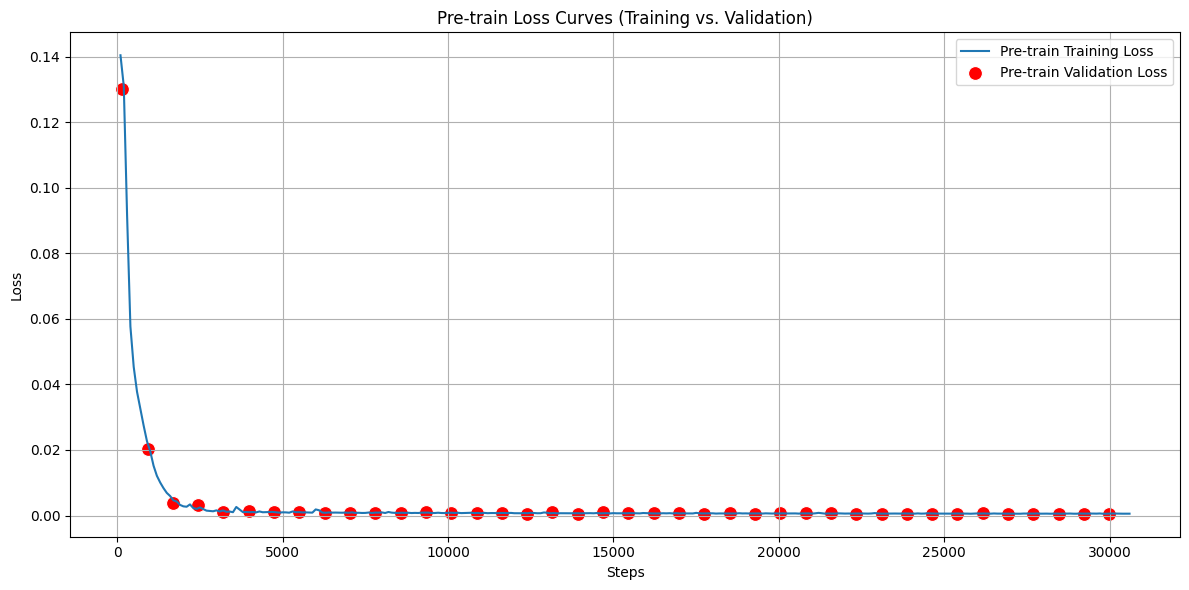
\includegraphics[width=\linewidth]{figures/pretrain_loss_curve.png}
    \caption{Unconditional pretraining loss curve.}
    \label{fig:pretrain_loss_curve}
\end{figure}

\begin{figure}[H]
  \centering
  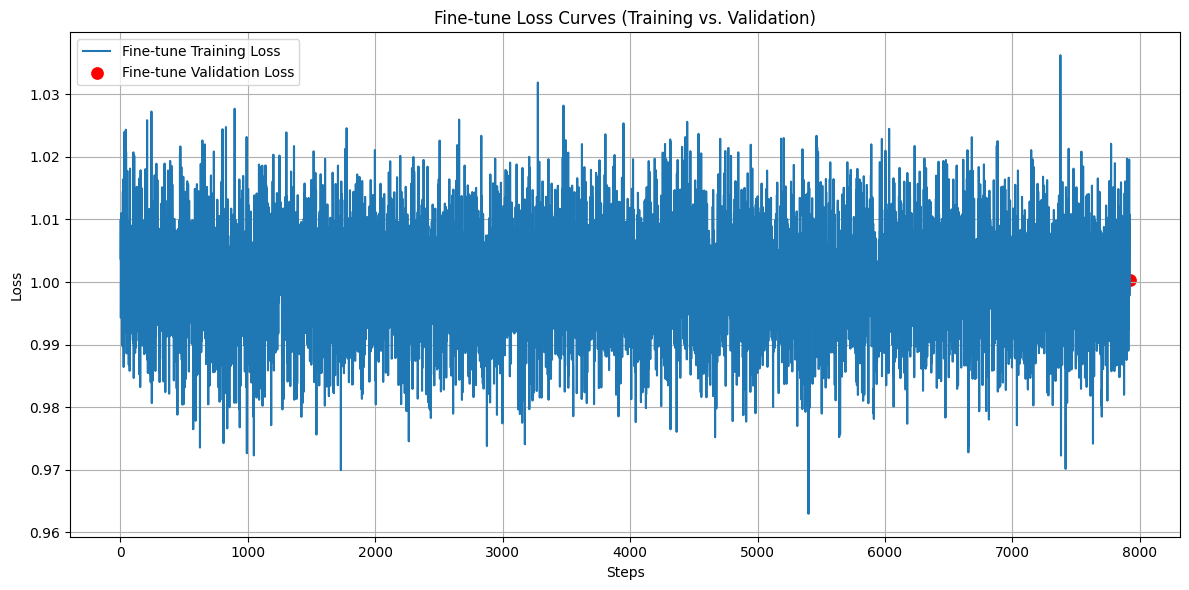
\includegraphics[width=\linewidth]{figures/finetune_mini_loss_curve.png}
    \caption{Fine-tuning loss curve.}
    \label{fig:finetune_loss_curve}
\end{figure}

\section{Proofs}
No additional formal proofs are included in this appendix.

\end{document}

